% Rapport de stage - Interface web de supervision et de commande AMR-X
% Compilation : latexmk -pdf -outdir=../../build/internship_dashboard_navigation main.tex
\documentclass[12pt,a4paper,oneside]{report}

\usepackage[utf8]{inputenc}
\usepackage[T1]{fontenc}
\usepackage{lmodern}
\usepackage[french]{babel}
\usepackage[a4paper,top=2.5cm,bottom=2.5cm,left=2.5cm,right=2.5cm,headheight=15pt]{geometry}
\usepackage{amsmath,amssymb}
\usepackage{graphicx}
\usepackage{booktabs,tabularx,multirow,longtable,array}
\usepackage[table]{xcolor}
\usepackage{caption,subcaption}
\usepackage{fancyhdr}
\usepackage{titlesec}
\usepackage{tocloft}
\usepackage{enumitem}
\usepackage{listings}
\usepackage{tikz}
\usetikzlibrary{arrows.meta,positioning,shapes.geometric,fit,calc,babel}
\usepackage{setspace}
\usepackage[hidelinks]{hyperref}

\setstretch{1.2}
\setlength{\parindent}{1.5em}
\setlength{\parskip}{0.4em}
\graphicspath{{figures/}}

% ---------------------------------------------------------------- numérotation
\renewcommand{\thechapter}{\Roman{chapter}}
\renewcommand{\thesection}{\arabic{section}}
\renewcommand{\thesubsection}{\arabic{section}.\arabic{subsection}}
\renewcommand{\thefigure}{\thechapter.\arabic{figure}}
\renewcommand{\thetable}{\thechapter.\arabic{table}}
\setcounter{secnumdepth}{3}
\setcounter{tocdepth}{2}

% ---------------------------------------------------------------- titres
\titleformat{\chapter}[display]
  {\normalfont\huge}{\chaptertitlename\ \thechapter}{1.2cm}{\Huge}
\titlespacing*{\chapter}{0pt}{2cm}{1.2cm}
\titleformat{\section}{\normalfont\Large\bfseries}{\thesection}{1em}{}
\titleformat{\subsection}{\normalfont\large\bfseries}{\thesubsection}{1em}{}
\captionsetup{labelsep=endash,font=small}
\captionsetup[figure]{name={\textsc{Figure}}}
\captionsetup[table]{name={\textsc{Tableau}}}

% ---------------------------------------------------------------- en-têtes
\pagestyle{fancy}
\fancyhf{}
\fancyhead[L]{\small\itshape\leftmark}
\fancyfoot[R]{\thepage}
\renewcommand{\headrulewidth}{0.4pt}
\renewcommand{\footrulewidth}{0.4pt}
\renewcommand{\chaptermark}[1]{\markboth{\chaptertitlename~\thechapter.\ #1}{}}
\fancypagestyle{plain}{\fancyhf{}\fancyfoot[C]{\thepage}%
  \renewcommand{\headrulewidth}{0pt}\renewcommand{\footrulewidth}{0pt}}

\renewcommand{\cfttoctitlefont}{\normalfont\Huge}
\renewcommand{\cftloftitlefont}{\normalfont\Huge}
\renewcommand{\cftlottitlefont}{\normalfont\Huge}
\renewcommand{\cftmarktoc}{\markboth{Table des matières}{}}
\renewcommand{\cftmarklof}{\markboth{Table des figures}{}}
\renewcommand{\cftmarklot}{\markboth{Liste des tableaux}{}}
\setlength{\emergencystretch}{3em}
\renewcommand{\topfraction}{0.9}
\renewcommand{\textfraction}{0.1}
\renewcommand{\floatpagefraction}{0.8}
\renewcommand{\cftdotsep}{1.5}
\renewcommand{\cftchapleader}{\hfill}

% ---------------------------------------------------------------- listings
\lstset{basicstyle=\ttfamily\small,columns=fullflexible,breaklines=true,
  frame=single,framerule=0.3pt,rulecolor=\color{gray!60},
  backgroundcolor=\color{gray!6},xleftmargin=0.5em,xrightmargin=0.5em,
  showstringspaces=false,upquote=true}

% ---------------------------------------------------------------- macros
% Valeur à compléter par l'auteur (organisme, encadrants, dates).
\newcommand{\acompleter}[1]{\textcolor{red!70!black}{[#1]}}
% Capture d'écran : insérée si le fichier existe dans figures/, sinon cadre réservé.
\newcommand{\capture}[3][0.9\linewidth]{%
  \IfFileExists{figures/#2}{\includegraphics[width=#1]{#2}}{%
    \fbox{\parbox[c][5.5cm][c]{#1}{\centering\small\itshape
      Capture à insérer : figures/#2\\[0.5em]\upshape #3}}}}
\newcommand{\code}[1]{\texttt{#1}}

% Style commun des schémas TikZ
\tikzset{
  bloc/.style={draw,rounded corners=3pt,thick,align=center,minimum height=1cm,
    inner sep=5pt,font=\small},
  web/.style={bloc,fill=blue!8},
  ros/.style={bloc,fill=orange!12},
  sim/.style={bloc,fill=green!10},
  neuf/.style={bloc,fill=red!8,draw=red!60!black,very thick},
  fl/.style={-{Stealth[length=2.5mm]},thick},
  lbl/.style={font=\scriptsize,align=center,fill=white,inner sep=1.5pt},
}

\begin{document}

% ---------------------------------------------------------------- page de garde
\begin{titlepage}
\thispagestyle{empty}
\begin{minipage}[c]{0.2\linewidth}
  \IfFileExists{figures/logo_insat.png}{\includegraphics[width=\linewidth]{logo_insat.png}}{}
\end{minipage}\hfill
\begin{minipage}[c]{0.58\linewidth}\centering
  {\bfseries RÉPUBLIQUE TUNISIENNE}\\[0.2em]
  Ministère de l'Enseignement Supérieur et de la Recherche Scientifique\\[0.2em]
  Université de Carthage\\[0.2em]
  Institut National des Sciences Appliquées et de Technologie
\end{minipage}\hfill
\begin{minipage}[c]{0.2\linewidth}
  \IfFileExists{figures/logo_carthage.png}{\includegraphics[width=\linewidth]{logo_carthage.png}}{}
\end{minipage}

\vspace{0.8cm}
\noindent\rule{\linewidth}{0.5pt}
\begin{center}
  {\Huge Rapport de stage d'été}\\[0.4em]
  {\large Spécialité : Informatique Industrielle et Automatique}
\end{center}
\noindent\rule{\linewidth}{0.5pt}

\begin{center}
  {\LARGE\bfseries Supervision et commande web\\[0.2em]
  du robot autonome modulaire AMR-X}\\[0.6em]
  {\large Intégration du dashboard avec la navigation Nav2\\
  et validation en simulation ROS~2 / Gazebo}
\end{center}
\noindent\rule{\linewidth}{0.5pt}

\vspace{0.6cm}
\begin{center}
  {\bfseries Réalisé par :}\\[0.2em]
  {\LARGE Linda Ouaghlani}\\[1em]
  Organisme d'accueil : \textbf{CyberMech Systems} -- département R\&D / Robotique\\[0.3em]
  Projet : \emph{Design, Development, Simulation, and Validation\\
  of a Modular Autonomous Robotic System}
  \IfFileExists{figures/logo_cybermech.png}{\\[0.8em]\includegraphics[height=1.8cm]{logo_cybermech.png}}{}
\end{center}

\vspace{0.6cm}
\begin{center}
\begin{tabular}{|p{0.5\linewidth}|}
  \hline
  \centering\bfseries Encadrant(e) à CyberMech Systems \tabularnewline
  \centering\acompleter{Nom et prénom} \tabularnewline[2.2cm]
  \hline
\end{tabular}
\end{center}

\vfill
\begin{center}
  Période du stage : du 1\textsuperscript{er} juillet au 31 août 2026\\[0.4em]
  {\bfseries Année universitaire : 2025\,/\,2026}
\end{center}
\end{titlepage}


\pagenumbering{roman}
% ---------------------------------------------------------------- remerciements
\chapter*{Remerciements}
\markboth{Remerciements}{}

Je tiens à remercier Monsieur \textbf{Hamza Abderrahmen}, directeur général de
\textbf{CyberMech Systems}, de m'avoir accueillie au sein du département R\&D / Robotique
pour ce stage d'été.

J'exprime ma gratitude à \acompleter{Nom de l'encadrant(e)}, mon encadrant(e) au sein de
CyberMech Systems, pour son accompagnement tout au long du stage, sa disponibilité et la
pertinence de ses retours.

Mes remerciements s'adressent aussi à l'ensemble de l'équipe du projet AMR-X, avec qui
j'ai eu le plaisir de travailler, ainsi qu'au corps professoral et administratif de l'INSAT
pour la formation reçue.

% ---------------------------------------------------------------- tables
\cleardoublepage
\renewcommand{\contentsname}{Table des matières}
\tableofcontents
\cleardoublepage
\renewcommand{\listfigurename}{Table des figures}
\listoffigures
\cleardoublepage
\renewcommand{\listtablename}{Liste des tableaux}
\listoftables

% ---------------------------------------------------------------- acronymes
\cleardoublepage
\chapter*{Liste des acronymes}
\addcontentsline{toc}{chapter}{Liste des acronymes}
\markboth{Liste des acronymes}{}
\begin{tabular}{@{}p{3cm}l@{}}
  \textbf{AMCL}   & Adaptive Monte Carlo Localization \\[0.3em]
  \textbf{AMR}    & Autonomous Mobile Robot \\[0.3em]
  \textbf{API}    & Application Programming Interface \\[0.3em]
  \textbf{JSON}   & JavaScript Object Notation \\[0.3em]
  \textbf{MPPI}   & Model Predictive Path Integral \\[0.3em]
  \textbf{Nav2}   & Navigation 2 (pile de navigation ROS~2) \\[0.3em]
  \textbf{QoS}    & Quality of Service \\[0.3em]
  \textbf{REST}   & Representational State Transfer \\[0.3em]
  \textbf{ROS 2}  & Robot Operating System 2 \\[0.3em]
  \textbf{RViz}   & ROS Visualization \\[0.3em]
  \textbf{SDF}    & Simulation Description Format \\[0.3em]
  \textbf{SLAM}   & Simultaneous Localization and Mapping \\[0.3em]
  \textbf{SPA}    & Single Page Application \\[0.3em]
  \textbf{SVG}    & Scalable Vector Graphics \\[0.3em]
  \textbf{TF}     & Transform (arbre des repères ROS) \\[0.3em]
  \textbf{UI}     & User Interface \\[0.3em]
\end{tabular}

% ---------------------------------------------------------------- glossaire
\cleardoublepage
\chapter*{Glossaire}
\addcontentsline{toc}{chapter}{Glossaire}
\markboth{Glossaire}{}
\begin{description}[style=nextline,leftmargin=4.8cm,labelwidth=4.5cm,font=\bfseries]
  \item[Acquittement] Réponse d'un service ROS indiquant que la demande a été reçue et
    acceptée ou refusée. Un acquittement positif ne signifie pas que la destination est
    atteinte.
  \item[Costmap] Grille d'occupation utilisée par Nav2, dont chaque cellule contient un
    coût de 0 (libre) à 100 (occupé) ou $-1$ (inconnu).
  \item[Dashboard] Application web existante du projet AMR-X, composée d'un frontend React
    et d'un backend FastAPI, servant à la supervision de la flotte.
  \item[Donnée périmée] État de navigation reçu depuis plus de 2,5~s ; le dashboard
    le considère comme non fiable et bloque toute nouvelle commande.
  \item[Monde SDF] Description de l'environnement simulé chargée par Gazebo ; le dashboard
    en extrait un plan 2D pour l'affichage.
  \item[Passerelle] Nœud ROS~2 \code{dashboard\_navigation} développé pendant le stage,
    intermédiaire unique entre le navigateur et Nav2.
  \item[Phase] État courant d'une demande de navigation :\\ \code{idle}, \code{sending},
    \code{navigating}, \code{canceling}, \code{succeeded},
    \code{canceled}, \code{failed} ou \code{rejected}.
  \item[Repère \code{map}] Repère global de Nav2, défini par la carte chargée. Il ne coïncide
    pas nécessairement avec le repère du monde Gazebo.
  \item[rosbridge] Serveur exposant les topics et services ROS~2 au navigateur à travers
    une connexion WebSocket (port 9090).
\end{description}


\cleardoublepage
\pagenumbering{arabic}
\chapter*{Introduction générale}
\addcontentsline{toc}{chapter}{Introduction générale}
\markboth{Introduction générale}{}

Un robot mobile autonome n'est exploitable que si un opérateur peut lui confier une tâche
et suivre son exécution. Dans un entrepôt ou un hôpital, cet opérateur ne travaille pas
dans un terminal ROS : il utilise une interface de supervision qui affiche la position des
robots, lui permet de désigner une destination et l'informe du résultat. La qualité de
cette interface dépend moins de son apparence que de la fidélité des informations
affichées : une position fausse, un ordre envoyé deux fois ou un succès annoncé à tort
peuvent conduire l'opérateur à une mauvaise décision.

Le présent stage s'inscrit dans le projet AMR-X, une plateforme de robot mobile modulaire
développée sous ROS~2. Au début du stage, le projet disposait déjà d'une simulation Gazebo
du robot dans un entrepôt, d'une pile de navigation Nav2 configurée et d'un dashboard web
de supervision. Ces trois briques fonctionnaient séparément : le dashboard affichait une
carte du monde mais ne pouvait ni connaître la position réelle du robot simulé, ni lui
envoyer une destination. L'objectif du stage est de relier ces briques afin que
l'opérateur puisse, depuis le dashboard, choisir une destination, commander le robot
simulé dans Gazebo et voir sa position et le résultat de la navigation dans le navigateur.

La démarche adoptée consiste d'abord à analyser l'existant et à définir un protocole de
communication sûr entre le navigateur et Nav2, puis à développer une passerelle ROS~2 et
les composants correspondants du dashboard, et enfin à valider l'ensemble dans la
simulation par des essais mesurés. Une attention particulière est portée à la cohérence
entre le repère de la carte Nav2 et celui du monde Gazebo, qui s'est révélée déterminante
lors des essais.

Ce rapport comporte quatre chapitres. Le premier présente le contexte du projet AMR-X,
l'existant, la problématique et le cahier des charges. Le deuxième décrit la conception de
la solution : architecture, protocole de communication, machine d'états et
transformation des repères. Le troisième détaille la réalisation de la passerelle ROS~2, de
l'interface web et de l'outillage de lancement, ainsi que les problèmes rencontrés. Le
quatrième présente le protocole de validation et les résultats mesurés en simulation.

\chapter{Contexte général du projet}

\section*{Introduction}
Ce chapitre situe le stage dans son environnement. Il présente d'abord l'organisme
d'accueil et le projet AMR-X, puis décrit les briques logicielles existantes au début du
stage et leurs limites. À partir de cet existant, la problématique et le cahier des charges
sont définis. Le chapitre se termine par l'environnement de travail et la démarche adoptée.

\section{Présentation de l'organisme d'accueil}
\acompleter{Présenter ici l'organisme d'accueil : activité, date de création,
implantation, équipe dans laquelle le stage a été réalisé.}

\section{Le projet AMR-X}
AMR-X (\emph{Autonomous Modular Robot -- Extended}) est un projet de plateforme mobile
modulaire : une base robotisée commune reçoit des modules fonctionnels interchangeables
selon l'application visée (logistique d'entrepôt, milieu hospitalier, etc.). Le dépôt du
projet regroupe la définition produit, les études de marché, la mécanique,
l'électronique, la partie robotique ROS~2 et les outils web.

La partie robotique cible l'environnement Ubuntu~24.04, ROS~2 Jazzy et Gazebo Harmonic.
Elle comprend notamment la description du robot, sa simulation dans plusieurs mondes
(entrepôt, hôpital), la cartographie par SLAM et la navigation autonome avec Nav2. Le
projet est mené par plusieurs équipes de stagiaires qui travaillent sur des parties
différentes du dépôt ; le travail présenté ici devait donc s'intégrer à l'existant sans le
reconstruire.

\section{Existant au début du stage}

\subsection{Simulation et navigation}
Le robot AMR-X est simulé dans Gazebo Harmonic. Le monde retenu pour ce stage est
l'entrepôt \code{warehouse\_harmonic}, dans lequel le robot apparaît à une position de
départ vérifiée, $(-1{,}2639 ; -3{,}9049)$~m. Le robot est équipé de deux LiDAR dont les
mesures sont fusionnées sur un topic unique, d'une caméra et d'une centrale inertielle.

La navigation repose sur Nav2 : localisation AMCL sur une carte d'occupation enregistrée
au préalable, planificateur global NavFn et contrôleur local MPPI. Une destination peut
être envoyée à Nav2 depuis RViz ou par l'action ROS~2 \code{/navigate\_to\_pose}.

\subsection{Dashboard web}
Le dashboard est une application web de supervision composée de deux parties :
\begin{itemize}
  \item un \textbf{frontend} React (Vite) organisé en pages : vue d'ensemble, robots,
    missions, carte en direct (\emph{Live map}), alertes, modules, téléopération,
    paramètres et gestion des utilisateurs ;
  \item un \textbf{backend} FastAPI avec SQLAlchemy et Alembic, qui gère les comptes (avec
    approbation par un administrateur), les robots, les missions et les alertes dans une
    base de données relationnelle.
\end{itemize}
La page \emph{Live map} affiche le monde SDF choisi sous forme de plan 2D (SVG) ou de vue
isométrique 3D. Les mondes sont extraits automatiquement des fichiers SDF du dépôt dans un
manifeste JSON (six mondes). Une connexion rosbridge existait déjà pour certaines pages.

\subsection{Limites de l'existant}
L'analyse de l'existant a fait apparaître les limites suivantes :
\begin{itemize}
  \item la \emph{Live map} n'affichait pas la position ROS du robot : les robots visibles
    provenaient de données de démonstration ou de la base de données ;
  \item en cas d'erreur de l'API, la page basculait implicitement sur les robots de
    démonstration, sans que l'utilisateur puisse distinguer des données réelles ;
  \item la vue 3D appliquait un décalage arbitraire de $(-12 ; -8)$ et animait un robot et
    un trajet décoratifs sans lien avec la simulation ;
  \item les boutons de la page \emph{Missions} enregistrent des missions dans la base mais
    ne pilotent pas Nav2 ;
  \item aucun chemin ne permettait d'envoyer une destination au robot depuis le navigateur
    ni d'en connaître le résultat.
\end{itemize}

\begin{figure}[htbp]
\centering
\begin{tikzpicture}[node distance=1.2cm and 1.6cm]
  \node[web,minimum width=4cm] (dash) {Dashboard web\\\scriptsize React + FastAPI};
  \node[web,below=0.5cm of dash,minimum width=4cm,fill=gray!10] (db)
    {Base de données\\\scriptsize robots, missions};
  \node[ros,right=3.6cm of dash,minimum width=3.6cm] (nav) {Nav2\\\scriptsize AMCL, NavFn, MPPI};
  \node[sim,below=0.5cm of nav,minimum width=3.6cm] (gz) {Gazebo Harmonic\\\scriptsize robot AMR-X simulé};
  \draw[fl] (dash) -- (db);
  \draw[fl] (nav) -- (gz);
  \draw[fl] (gz.east) -- ++(0.5,0) |- node[lbl,pos=0.25]{capteurs} (nav.east);
  \draw[thick,dashed,red!70!black] (dash.east) -- node[lbl,text=red!70!black]{aucun lien\\
    position / commande} (nav.west);
  \node[font=\scriptsize\itshape,below=0.2cm of db] {affichage : démo ou base de données};
  \node[font=\scriptsize\itshape,below=0.2cm of gz] {commande : RViz uniquement};
\end{tikzpicture}
\caption{Briques existantes au début du stage.}
\label{fig:existant}
\end{figure}

\section{Problématique}
Le dashboard et la simulation formaient deux mondes séparés. La problématique du stage
peut se formuler ainsi : \emph{comment permettre à un opérateur de commander la navigation
du robot AMR-X simulé depuis le dashboard web existant, tout en lui garantissant que la
position et l'état affichés correspondent réellement à ceux du robot ?}

Plusieurs difficultés en découlent. Le navigateur communique en WebSocket et ne parle pas
directement ROS~2. Une commande envoyée à travers le réseau peut être perdue, dupliquée ou
arriver alors que le robot exécute déjà une autre destination. Le plan affiché dans le
navigateur est construit à partir du monde SDF de Gazebo, alors que Nav2 raisonne dans le
repère de sa carte. Enfin, l'interface doit rester honnête lorsque les données deviennent
indisponibles, par exemple si la simulation est en pause ou si la connexion est perdue.

\section{Cahier des charges}

\subsection{Besoins fonctionnels}
Le tableau~\ref{tab:besoins} résume les besoins fonctionnels retenus.

\begin{table}[htbp]
\centering\small
\begin{tabularx}{\linewidth}{@{}lX@{}}
\toprule
\textbf{Réf.} & \textbf{Besoin} \\
\midrule
BF1 & Afficher en direct la position et l'orientation du robot simulé sur la \emph{Live map} (vues 2D et 3D). \\
BF2 & Choisir une destination par clic sur la carte 2D ou par saisie de X, Y (m) et du cap (°). \\
BF3 & Envoyer la destination à Nav2 et obtenir un acquittement explicite de la demande. \\
BF4 & Suivre l'état de la navigation : envoi, navigation, distance restante, résultat final. \\
BF5 & Annuler la navigation en cours et afficher la confirmation d'annulation. \\
BF6 & Refuser les destinations invalides (hors carte, occupées, non finies, mauvais monde) avec un message explicite. \\
\bottomrule
\end{tabularx}
\caption{Besoins fonctionnels.}
\label{tab:besoins}
\end{table}

\subsection{Besoins non fonctionnels}
\begin{itemize}
  \item \textbf{Fidélité} : ne jamais afficher de position ou de résultat inventé ; le
    succès provient uniquement du résultat Nav2.
  \item \textbf{Sûreté des commandes} : un seul but actif à la fois, pas de renvoi
    automatique d'une commande dont le résultat est incertain.
  \item \textbf{Détection des données périmées} : bloquer les commandes si l'état n'a pas
    été reçu depuis 2,5~s.
  \item \textbf{Intégration} : réutiliser le dashboard, Nav2 et la simulation existants
    sans les reconstruire ; conserver l'authentification existante.
  \item \textbf{Reproductibilité} : pouvoir lancer et vérifier l'ensemble de la chaîne
    par des commandes documentées.
\end{itemize}

\subsection{Périmètre et limites}
Le périmètre a été volontairement restreint à un robot, un serveur de navigation et un
monde actif à la fois. Le travail porte sur la simulation : la passerelle refuse les
destinations lorsque le temps simulé n'est pas utilisé, afin d'éviter toute commande
d'un robot physique. La pause et la reprise d'une navigation, l'arbitrage avec d'autres
sources de commande (RViz, téléopération) et l'authentification des commandes au niveau de
rosbridge sont hors périmètre. Les navigations lancées depuis la \emph{Live map} ne sont
pas enregistrées dans la base de données.

\section{Environnement de travail}
Le tableau~\ref{tab:env} présente les outils utilisés.

\begin{table}[htbp]
\centering\small
\begin{tabular}{@{}ll@{}}
\toprule
\textbf{Élément} & \textbf{Version / outil} \\
\midrule
Système d'exploitation & Ubuntu 24.04 \\
Intergiciel robotique & ROS~2 Jazzy \\
Simulateur & Gazebo Harmonic \\
Navigation & Nav2 (AMCL, NavFn, MPPI) \\
Pont web & rosbridge\_server 2.7.1 (WebSocket, port 9090) \\
Frontend & React 19, Vite 8, roslib 2.1 \\
Backend & FastAPI, SQLAlchemy, Alembic \\
Environnement JavaScript & Node.js 20 \\
Gestion de version & Git, GitHub \\
\bottomrule
\end{tabular}
\caption{Environnement logiciel du stage.}
\label{tab:env}
\end{table}

\section{Démarche adoptée}
Le travail a été conduit en quatre étapes :
\begin{enumerate}
  \item analyse de l'existant (dashboard, simulation, configuration Nav2) et définition du
    parcours utilisateur ;
  \item conception du protocole entre le navigateur et Nav2 et de la gestion des repères ;
  \item développement de la passerelle ROS~2 et des composants du dashboard, avec des tests
    unitaires sans ROS ;
  \item intégration sous Ubuntu, correction des problèmes observés et validation par des
    essais mesurés dans Gazebo.
\end{enumerate}

\section*{Conclusion}
Ce chapitre a présenté le projet AMR-X et l'existant au début du stage : une simulation,
une pile Nav2 et un dashboard fonctionnels mais non reliés. Le cahier des charges fixe
l'objectif de commander le robot depuis le dashboard avec des informations fidèles. Le
chapitre suivant décrit la conception retenue pour y parvenir.

\chapter{Conception de la solution}

\section*{Introduction}
Ce chapitre présente la conception retenue pour relier le dashboard à Nav2. Il décrit
l'architecture générale, justifie le choix d'une passerelle ROS~2 dédiée, puis détaille le
protocole de communication, la machine d'états d'une demande de navigation, la gestion
des repères et les règles de sûreté.

\section{Architecture générale}
La figure~\ref{fig:architecture} présente la chaîne retenue. Le navigateur communique avec
ROS~2 par rosbridge, au moyen d'une connexion WebSocket. Il n'appelle pas Nav2
directement : toutes les commandes passent par un nœud intermédiaire,
\code{dashboard\_navigation}, qui vérifie la demande, dialogue avec Nav2 par l'action
\code{/navigate\_to\_pose} et publie en retour un état synthétique. La position du robot
est lue dans l'arbre TF (transformation \code{map}~$\rightarrow$~\code{base\_link}), qui
combine la localisation AMCL et l'odométrie.

\begin{figure}[htbp]
\centering
\resizebox{\linewidth}{!}{%
\begin{tikzpicture}[node distance=0.9cm and 1.1cm]
  \node[web,minimum width=3.4cm] (ui) {Live Map (React)\\\scriptsize NavigationPanel\\\scriptsize useNavigation};
  \node[ros,right=1.6cm of ui,minimum width=2.6cm] (rb) {rosbridge\\\scriptsize WebSocket :9090};
  \node[neuf,right=1.6cm of rb,minimum width=3.4cm] (gw) {Passerelle\\\code{dashboard\_navigation}};
  \node[ros,right=1.6cm of gw,minimum width=2.6cm] (nav) {Nav2\\\scriptsize bt\_navigator};
  \node[sim,below=1.5cm of nav,minimum width=2.6cm] (gz) {Gazebo\\\scriptsize robot simulé};
  \node[ros,below=1.5cm of gw,minimum width=3.4cm] (tf) {TF \code{map}$\rightarrow$\code{base\_link}\\\scriptsize + costmap globale};
  \node[web,below=1.5cm of ui,minimum width=3.4cm,fill=gray!10] (api) {Backend FastAPI\\\scriptsize comptes, flotte};
  \draw[fl] ([yshift=2mm]ui.east) -- node[lbl,above=1pt]{services} ([yshift=2mm]rb.west);
  \draw[fl] ([yshift=-2mm]rb.west) -- node[lbl,below=1pt]{état JSON} ([yshift=-2mm]ui.east);
  \draw[fl] ([yshift=2mm]rb.east) -- node[lbl,above=1pt]{submit / cancel} ([yshift=2mm]gw.west);
  \draw[fl] ([yshift=-2mm]gw.west) -- node[lbl,below=1pt]{4 Hz} ([yshift=-2mm]rb.east);
  \draw[fl] ([yshift=2mm]gw.east) -- node[lbl,above=1pt]{action} ([yshift=2mm]nav.west);
  \draw[fl] ([yshift=-2mm]nav.west) -- node[lbl,below=1pt]{retour} ([yshift=-2mm]gw.east);
  \draw[fl] (nav) -- node[lbl]{\code{cmd\_vel}} (gz);
  \draw[fl] (gz) -- node[lbl]{capteurs, AMCL} (tf);
  \draw[fl] (tf) -- node[lbl]{pose, coûts} (gw);
  \draw[fl] (ui) -- node[lbl]{HTTP REST} (api);
\end{tikzpicture}}
\caption{Architecture de la chaîne de commande et de retour (en rouge, le nœud développé).}
\label{fig:architecture}
\end{figure}

\section{Choix d'une passerelle dédiée}
Deux approches étaient possibles pour envoyer une destination depuis le navigateur :
publier directement un message sur le topic \code{/goal\_pose} ou appeler l'action Nav2
depuis le navigateur, ou bien passer par un nœud intermédiaire. La première approche est
simple mais ne fournit aucun accusé de réception : le navigateur ne sait pas si la commande
a été reçue, refusée ou perdue. La seconde place dans le navigateur toute la logique de
vérification, qui peut alors être contournée ou dupliquée par plusieurs onglets.

La passerelle dédiée a été retenue pour les raisons suivantes :
\begin{itemize}
  \item chaque commande reçoit une réponse explicite (\emph{acceptée} ou \emph{refusée}
    avec un motif) ;
  \item les vérifications (monde, coordonnées, carte, disponibilité de Nav2) sont faites
    côté ROS, au plus près des données ;
  \item un seul but peut être actif à la fois, quel que soit le nombre de navigateurs ;
  \item l'état publié est unique et partagé : tous les clients voient la même information.
\end{itemize}

\section{Protocole de communication}

\subsection{Service de soumission}
La soumission utilise une interface de service dédiée, définie dans le paquet
\code{navigation\_msgs} :
\begin{lstlisting}
# Coordinates in the dashboard's configured SDF world (metres, radians).
string request_id
string world_id
float64 x
float64 y
float64 yaw
---
bool accepted
string message
\end{lstlisting}
Le champ \code{request\_id} est un identifiant aléatoire de 32 caractères hexadécimaux
généré par le navigateur. Il permet à la passerelle de reconnaître une demande déjà reçue
et de ne pas l'exécuter deux fois. Le champ \code{world\_id} identifie le monde affiché dans
le dashboard ; la passerelle refuse la demande s'il ne correspond pas au monde simulé.
L'annulation utilise le service standard \code{std\_srvs/srv/Trigger}.

Un acquittement positif signifie uniquement \og demande reçue et transmise à Nav2 \fg{}. Le
résultat réel de la navigation n'est connu qu'à travers l'état publié.

\subsection{État de navigation}
La passerelle publie à 4~Hz sur \code{/dashboard/navigation/state} un message
\code{std\_msgs/String} contenant un objet JSON versionné (tableau~\ref{tab:etat}). Ce
choix évite de créer un type de message supplémentaire côté navigateur tout en gardant un
format validé strictement par le frontend.

\begin{table}[htbp]
\centering\small
\begin{tabularx}{\linewidth}{@{}lX@{}}
\toprule
\textbf{Champ} & \textbf{Contenu} \\
\midrule
\code{version} & Version du format (1) ; toute autre valeur est rejetée par le frontend. \\
\code{world\_id} & Monde configuré sur la passerelle. \\
\code{request\_id} & Identifiant de la dernière demande acceptée. \\
\code{phase}, \code{detail} & Phase de la demande et message lisible. \\
\code{ready}, \code{unavailable\_reason} & Disponibilité pour une nouvelle destination et motif sinon. \\
\code{pose} & Position $(x, y)$ et cap du robot dans le repère du monde, ou \code{null}. \\
\code{target} & Destination en cours, dans le repère du monde. \\
\code{distance\_remaining} & Distance restante fournie par le retour de Nav2. \\
\bottomrule
\end{tabularx}
\caption{Contenu de l'état de navigation publié par la passerelle.}
\label{tab:etat}
\end{table}

\subsection{Séquence d'une navigation}
La figure~\ref{fig:sequence} montre les échanges lors d'une navigation réussie.

\begin{figure}[htbp]
\centering
\begin{tikzpicture}[y=-0.62cm]
  \foreach \x/\n in {0/Navigateur,3.6/Passerelle,7.2/Nav2,10.4/Gazebo}{
    \node[bloc,fill=gray!8,minimum width=2.4cm] at (\x,0) {\n};
    \draw[gray,dashed] (\x,0.8) -- (\x,12.2);}
  \draw[fl] (0,1.5) -- node[lbl,above]{submit(request\_id, x, y, cap)} (3.6,1.5);
  \node[font=\scriptsize\itshape,align=left,anchor=east] at (3.5,2.4) {vérifications};
  \draw[fl] (3.6,3.2) -- node[lbl,above]{send\_goal} (7.2,3.2);
  \draw[fl,dashed] (3.6,3.9) -- node[lbl,above]{accepted = true} (0,3.9);
  \draw[fl,dashed] (7.2,4.8) -- node[lbl,above]{but accepté} (3.6,4.8);
  \draw[fl] (7.2,5.6) -- node[lbl,above]{cmd\_vel} (10.4,5.6);
  \draw[fl,dashed] (7.2,6.6) -- node[lbl,above]{feedback (distance)} (3.6,6.6);
  \draw[fl,dashed] (3.6,7.4) -- node[lbl,above]{état : navigating} (0,7.4);
  \draw[fl,dashed] (7.2,9.2) -- node[lbl,above]{résultat : SUCCEEDED} (3.6,9.2);
  \draw[fl,dashed] (3.6,10.2) -- node[lbl,above]{état : succeeded} (0,10.2);
  \node[font=\scriptsize\itshape,anchor=west] at (3.7,11.3) {état publié à 4 Hz en continu};
\end{tikzpicture}
\caption{Séquence d'une navigation réussie.}
\label{fig:sequence}
\end{figure}

\section{Machine d'états d'une demande}
Chaque demande suit la machine d'états de la figure~\ref{fig:etats}. Les phases
\code{sending}, \code{navigating} et \code{canceling} sont dites \emph{actives} : pendant
ces phases, toute nouvelle destination est refusée. Une annulation demandée pendant la
phase \code{sending}, avant l'acceptation par Nav2, est mémorisée et transmise dès que le
but est accepté. Si Nav2 refuse l'annulation, la phase revient à \code{navigating} avec un
message explicite, afin de ne jamais laisser croire que le robot s'est arrêté.

\begin{figure}[htbp]
\centering
\begin{tikzpicture}[st/.style={bloc,rounded corners=8pt,minimum width=2.2cm},
  node distance=1.1cm and 1.5cm]
  \node[st] (idle) {idle};
  \node[st,fill=yellow!15,right=of idle] (send) {sending};
  \node[st,fill=yellow!15,right=of send] (nav) {navigating};
  \node[st,fill=yellow!15,below=1.4cm of nav] (can) {canceling};
  \node[st,fill=green!15,right=1.3cm of nav] (ok) {succeeded};
  \node[st,fill=red!10,above=1.1cm of nav] (fail) {failed};
  \node[st,fill=red!10,above=1.1cm of send] (rej) {rejected};
  \node[st,fill=gray!15,right=1.3cm of can] (cand) {canceled};
  \draw[fl] (idle) -- node[lbl,above]{submit} (send);
  \draw[fl] (send) -- node[lbl,above]{accepté} (nav);
  \draw[fl] (send) -- node[lbl,left]{refusé} (rej);
  \draw[fl] (nav) -- node[lbl,above]{succès} (ok);
  \draw[fl] (nav) -- node[lbl,left]{échec} (fail);
  \draw[fl] (nav) -- node[lbl,left]{cancel} (can);
  \draw[fl] (send) |- node[lbl,pos=0.3,left]{cancel} (can);
  \draw[fl] (can) -- node[lbl,above]{annulé} (cand);
\end{tikzpicture}
\caption{Phases d'une demande de navigation (en jaune, les phases actives).}
\label{fig:etats}
\end{figure}

\section{Gestion des repères}
Le dashboard dessine le monde à partir du fichier SDF de Gazebo ; ses coordonnées sont
donc celles du monde simulé. Nav2, lui, travaille dans le repère \code{map} défini par la
carte chargée. Ces deux repères ne coïncident pas nécessairement : une carte construite par
SLAM a pour origine la position du robot au début de l'enregistrement.

La passerelle est configurée par la pose de l'origine du repère \code{map} dans le monde,
notée $(t_x, t_y, \theta)$ (paramètres \code{world\_offset\_x}, \code{world\_offset\_y},
\code{world\_offset\_yaw}). La conversion d'une pose de la carte vers le monde est :
\begin{equation}
\begin{pmatrix} x_w \\ y_w \end{pmatrix} =
\begin{pmatrix} \cos\theta & -\sin\theta \\ \sin\theta & \cos\theta \end{pmatrix}
\begin{pmatrix} x_m \\ y_m \end{pmatrix} +
\begin{pmatrix} t_x \\ t_y \end{pmatrix},
\qquad \psi_w = \psi_m + \theta,
\label{eq:map2world}
\end{equation}
où $(x_m, y_m, \psi_m)$ est la pose dans \code{map} et $(x_w, y_w, \psi_w)$ la pose dans
le monde. Une destination choisie dans le dashboard est convertie par la transformation
inverse avant d'être envoyée à Nav2 :
\begin{equation}
\begin{pmatrix} x_m \\ y_m \end{pmatrix} =
\begin{pmatrix} \cos\theta & \sin\theta \\ -\sin\theta & \cos\theta \end{pmatrix}
\begin{pmatrix} x_w - t_x \\ y_w - t_y \end{pmatrix},
\qquad \psi_m = \psi_w - \theta.
\label{eq:world2map}
\end{equation}
Le cap est manipulé en radians côté ROS et saisi en degrés dans l'interface. La position
du robot est toujours lue par TF dans le repère \code{map}, jamais à partir de l'odométrie
seule, qui dérive.

\section{Vérification des destinations}
Avant d'envoyer un but à Nav2, la passerelle consulte la costmap globale. La destination,
convertie dans \code{map}, est ramenée dans le repère de la grille (origine et rotation de
la grille), puis la cellule est obtenue par
\begin{equation}
  i = \left\lfloor \frac{g_x}{r} \right\rfloor, \qquad
  j = \left\lfloor \frac{g_y}{r} \right\rfloor,
\end{equation}
où $(g_x, g_y)$ sont les coordonnées dans la grille et $r$ sa résolution. L'arrondi par
défaut (et non la troncature) garantit qu'un point situé juste avant un bord négatif est
bien considéré comme hors de la grille. La destination est refusée si la cellule est hors
carte, inconnue ($-1$) ou si son coût atteint le seuil d'occupation de 65 (sur une échelle
de 0 à 100). La carte approximative dessinée par le dashboard n'est jamais utilisée pour ce
contrôle. Une cellule libre peut toutefois être inaccessible : dans ce cas, c'est Nav2 qui
renvoie un échec, et l'interface l'affiche sans le transformer.

\section{Règles de sûreté et de fraîcheur}
Le tableau~\ref{tab:regles} résume les règles appliquées de part et d'autre.

\begin{table}[htbp]
\centering\small
\begin{tabularx}{\linewidth}{@{}lX@{}}
\toprule
\textbf{Côté} & \textbf{Règle} \\
\midrule
Passerelle & Refus si le temps simulé n'est pas utilisé (\code{use\_sim\_time} faux). \\
Passerelle & Refus si Nav2 est absent, si la transformation TF a plus de 2~s ou si la costmap a plus de 5~s. \\
Passerelle & Un seul but actif ; un \code{request\_id} déjà reçu n'est jamais réexécuté. \\
Passerelle & Horloge de publication basée sur le temps simulé : l'état n'est plus publié si Gazebo est en pause. \\
Dashboard & État considéré périmé après 2,5~s : position retirée de la carte et commandes bloquées. \\
Dashboard & Commandes interdites en mode démonstration ou si le monde affiché diffère du monde simulé. \\
Dashboard & Délai d'acquittement de 6~s ; en cas d'expiration, aucun renvoi automatique et message invitant à consulter l'état. \\
\bottomrule
\end{tabularx}
\caption{Règles de sûreté et de fraîcheur des données.}
\label{tab:regles}
\end{table}

\section*{Conclusion}
La conception repose sur une passerelle ROS~2 unique, un protocole acquitté et un état
publié en continu, ainsi que sur une conversion explicite entre le repère de la carte et
celui du monde. Le chapitre suivant présente la réalisation de ces éléments.

\chapter{Réalisation}

\section*{Introduction}
Ce chapitre décrit la mise en œuvre de la conception : les paquets ROS~2 ajoutés ou
modifiés, la passerelle de navigation, les composants du dashboard, l'outillage de
lancement et les tests automatisés.

\section{Organisation des fichiers}
Le travail s'insère dans le dépôt existant. Le tableau~\ref{tab:fichiers} liste les
principaux fichiers ajoutés.

\begin{table}[!htb]
\centering\footnotesize
\begin{tabularx}{\linewidth}{@{}>{\ttfamily\raggedright\arraybackslash}p{7.4cm}X@{}}
\toprule
\normalfont\textbf{Fichier} & \textbf{Rôle} \\
\midrule
navigation\_msgs/srv/ SubmitNavigationGoal.srv & Interface du service de soumission. \\
navigation/scripts/ dashboard\_navigation\_node.py & Passerelle : services, action Nav2, TF, état JSON. \\
navigation/scripts/ dashboard\_navigation\_math.py & Conversions de repères et lecture de la costmap, sans dépendance ROS. \\
navigation/launch/ dashboard\_navigation.launch.py & Lancement de la passerelle et, en option, de rosbridge. \\
navigation/test/ test\_dashboard\_navigation\_math.py & Tests unitaires Python des conversions. \\
frontend/src/hooks/ useNavigation.js & Abonnement à l'état, fraîcheur, appels de services. \\
frontend/src/utils/ navigation.js & Validation du protocole et conditions d'envoi. \\
frontend/src/components/ NavigationPanel.jsx & Panneau de destination, d'état et d'annulation. \\
frontend/tests/ navigation.test.mjs & Tests unitaires JavaScript. \\
scripts/run-all.sh & Lancement de toute la chaîne en une commande. \\
\bottomrule
\end{tabularx}
\caption{Principaux fichiers ajoutés.}
\label{tab:fichiers}
\end{table}

Les fichiers existants modifiés sont principalement les \code{CMakeLists.txt} et
\code{package.xml} des paquets \code{navigation} et \code{navigation\_msgs} (génération de
l'interface, installation des scripts, dépendances), la page \code{Map.jsx}, les
composants de carte 2D et 3D, le hook de connexion ROS et la page des paramètres.

\section{Passerelle ROS~2}

\subsection{Paramètres}
La passerelle est un nœud Python (\code{rclpy}). Ses paramètres sont donnés dans le
tableau~\ref{tab:params}.

\begin{table}[htbp]
\centering\small
\begin{tabular}{@{}lll@{}}
\toprule
\textbf{Paramètre} & \textbf{Défaut} & \textbf{Rôle} \\
\midrule
\code{world\_id} & -- & Monde du dashboard correspondant à la simulation \\
\code{base\_frame} & \code{base\_link} & Repère du robot lu dans TF \\
\code{world\_offset\_x}, \code{\_y} & 0,0 & Position de l'origine de \code{map} dans le monde (m) \\
\code{world\_offset\_yaw} & 0,0 & Rotation de \code{map} dans le monde (rad) \\
\code{occupied\_threshold} & 65 & Seuil de coût d'une cellule occupée \\
\code{use\_sim\_time} & \code{true} & Imposé par le fichier de lancement \\
\bottomrule
\end{tabular}
\caption{Paramètres de la passerelle.}
\label{tab:params}
\end{table}

\subsection{Fonctionnement}
Le nœud s'abonne à la costmap globale avec une qualité de service \emph{transient local},
identique à celle de l'éditeur Nav2, afin de recevoir la dernière grille même s'il démarre
après Nav2. Un temporisateur de 0,25~s calcule à chaque cycle la pose du robot et la
disponibilité, puis publie l'état. Les principaux traitements sont :
\begin{itemize}
  \item \textbf{soumission} : contrôle de l'identifiant, du but actif, du monde, des
    coordonnées, de la disponibilité, conversion par l'équation~\eqref{eq:world2map}, contrôle
    de la cellule, puis envoi asynchrone du but à Nav2 ;
  \item \textbf{acceptation} : à la réponse de Nav2, passage en \code{navigating} ou en
    \code{rejected}, et envoi d'une annulation mémorisée le cas échéant ;
  \item \textbf{retour} : mise à jour de la distance restante ;
  \item \textbf{résultat} : conversion du statut Nav2 en \code{succeeded},
    \code{canceled} ou \code{failed} ;
  \item \textbf{annulation} : passage en \code{canceling} et demande d'annulation à Nav2 ;
    la phase terminale n'est affichée qu'à réception du résultat.
\end{itemize}
Les calculs de repères et de cellules sont isolés dans un module Python sans dépendance
ROS, ce qui permet de les tester sans lancer de simulation.

\subsection{Fichier de lancement}
Le fichier \code{dashboard\_navigation.launch.py} démarre la passerelle avec
\code{use\_sim\_time} et inclut le serveur rosbridge, sauf si l'argument
\code{start\_rosbridge:=false} est donné. Les décalages de repère sont passés en arguments :
\begin{lstlisting}
ros2 launch navigation dashboard_navigation.launch.py \
  world_id:=warehouse-harmonic \
  world_offset_x:=-1.2639 world_offset_y:=-3.9049 world_offset_yaw:=0.0
\end{lstlisting}

\section{Interface web}

\subsection{Logique de navigation}
Le hook React \code{useNavigation} s'abonne à l'état publié par la passerelle au moyen de
\code{roslib}. Chaque message est validé par \code{parseNavigationState} : version,
types des champs, phase connue et pose finie. Un message non conforme n'est pas affiché
comme une donnée réelle. L'âge du dernier message est réévalué toutes les 0,5~s ; au-delà
de 2,5~s, l'état est considéré périmé.

La fonction \code{navigationBlockReason} centralise les conditions d'envoi et retourne le
motif de blocage à afficher (mode démonstration, déconnexion, données périmées, mauvais
monde, passerelle non prête, but actif). Elle est réévaluée au moment exact du clic, et
non seulement au dernier rendu. Un seul appel de service peut être en attente ; en
l'absence de réponse sous 6~s, l'interface signale que le résultat est incertain et ne
renvoie pas la commande.

\subsection{Panneau de navigation et carte}
Le composant \code{NavigationPanel} affiche la phase et son
détail, la distance restante, le motif de blocage éventuel et les erreurs. L'opérateur
choisit une destination en cliquant sur la carte 2D après avoir activé \emph{Choose on
map}, ou en saisissant X et Y en mètres et le cap en degrés. Les boutons \emph{Go to
destination} et \emph{Cancel navigation} ne sont actifs que lorsque l'action est permise.
Un message rappelle que fermer la page n'annule pas la navigation.

La page \emph{Live map} a été adaptée (figure~\ref{fig:livemap}) :
\begin{itemize}
  \item le robot est dessiné à partir de la pose ROS uniquement lorsque l'état est frais
    et que le monde correspond ; la pose de la base de données n'est plus utilisée en
    remplacement ;
  \item un marqueur indique la destination choisie ;
  \item le mode démonstration est signalé explicitement et une erreur de l'API n'active
    plus implicitement les robots de démonstration ;
  \item la projection du robot et du trajet sur le plan 2D utilise la même transformation
    que le monde SDF, et l'orientation ROS est convertie pour le repère SVG ;
  \item la vue 3D n'applique plus de décalage arbitraire et oriente le robot selon sa pose ;
    le robot et le trajet décoratifs ont été supprimés.
\end{itemize}
\begin{figure}[htbp]
\centering
\capture{live_map_navigation.png}{Page Live map.}
\caption{Page \emph{Live map} : robot \code{amr\_x} affiché à sa position ROS sur le plan
du monde \code{warehouse\_harmonic}.}
\label{fig:livemap}
\end{figure}

Enfin, la connexion rosbridge se rétablit automatiquement après une fermeture du
WebSocket, et une nouvelle adresse saisie dans \emph{Settings} est appliquée sans
recharger la page.

\section{Lancement de la chaîne complète}
La chaîne complète comporte cinq processus : simulation, Nav2, passerelle avec rosbridge,
backend et frontend. Pour la rendre reproductible, un script \code{scripts/run-all.sh} les
démarre dans l'ordre, attend que chacun soit prêt avant de lancer le suivant, et arrête
l'ensemble par un simple \emph{Ctrl+C} (figure~\ref{fig:lancement}). Il envoie également la
pose initiale à AMCL, ce qui évite une intervention manuelle dans RViz.

\begin{lstlisting}
cd amr
bash scripts/run-all.sh          # fenetre Gazebo ouverte
bash scripts/run-all.sh rviz     # avec RViz en plus
\end{lstlisting}

\begin{figure}[htbp]
\centering
\resizebox{\linewidth}{!}{%
\begin{tikzpicture}[node distance=0.55cm]
  \node[sim] (a) {1. Gazebo\\\scriptsize attente \code{/clock}};
  \node[ros,right=of a] (b) {2. Nav2\\\scriptsize attente AMCL actif};
  \node[ros,right=of b] (c) {pose initiale\\\scriptsize \code{/initialpose}};
  \node[neuf,right=of c] (d) {3. Passerelle\\\scriptsize attente \code{ready}};
  \node[web,right=of d] (e) {4. Backend\\\scriptsize :8000};
  \node[web,right=of e] (f) {5. Frontend\\\scriptsize :5173};
  \draw[fl] (a) -- (b); \draw[fl] (b) -- (c); \draw[fl] (c) -- (d);
  \draw[fl] (d) -- (e); \draw[fl] (e) -- (f);
\end{tikzpicture}}
\caption{Séquence de démarrage du script \code{run-all.sh}.}
\label{fig:lancement}
\end{figure}

\section{Tests automatisés}
Deux jeux de tests unitaires ne nécessitent ni ROS ni Gazebo :
\begin{itemize}
  \item \textbf{Python} (5 tests) : aller-retour entre les repères, repère carte tourné,
    cellules occupées, inconnues et hors carte, grille d'origine tournée, grille invalide ;
  \item \textbf{JavaScript} (5 tests) : conditions d'envoi, blocage des buts concurrents,
    rejet des états mal formés, validité des coordonnées nulles ou négatives,
    unicité et format des identifiants de requête.
\end{itemize}
Un test navigateur optionnel, fondé sur Playwright et un faux serveur rosbridge, vérifie
en plus le parcours complet de l'interface (envoi, conversion degrés/radians, annulation,
sélection sur la carte, blocage d'un mauvais monde). Il ne remplace pas les essais dans
Gazebo présentés au chapitre suivant.

\section*{Conclusion}
La passerelle, l'interface web et l'outillage de lancement ont été réalisés et intégrés
à l'environnement du projet. Les tests unitaires couvrent les conversions de repères et la logique de
l'interface. Il reste à vérifier le comportement de l'ensemble dans la simulation, ce qui
fait l'objet du chapitre suivant.

\chapter{Validation en simulation}
\label{chap:validation}

\section*{Introduction}
Ce chapitre présente la validation de la chaîne complète dans Gazebo. Il décrit
l'environnement et la méthode d'essai, puis les vérifications préalables. Il expose
ensuite le décalage de repères mis en évidence par les premiers essais et sa correction,
avant de présenter les résultats mesurés après correction et les points qui restent à
valider. Toutes les valeurs données sont issues de mesures réalisées le 29~septembre~2026.

\section{Environnement et méthode d'essai}
Les essais ont été réalisés sur un poste Ubuntu~24.04 avec ROS~2 Jazzy et Gazebo Harmonic,
dans le monde \code{warehouse\_harmonic}, avec la carte \code{warehouse\_harmonic.yaml}.
La chaîne complète était lancée par \code{scripts/run-all.sh}, fenêtre Gazebo ouverte
(figure~\ref{fig:gazebo}).

\begin{figure}[htbp]
\centering
\capture{gazebo_warehouse.png}{Fenêtre Gazebo : robot AMR-X dans l'entrepôt warehouse\_harmonic.}
\caption{Robot AMR-X simulé dans l'entrepôt Gazebo.}
\label{fig:gazebo}
\end{figure}

Pour obtenir des mesures reproductibles, les scénarios de navigation ont été pilotés par
un script de test qui appelle \emph{les mêmes services} que le dashboard,
\code{/dashboard/navigation/submit} et \code{/dashboard/navigation/cancel}, et enregistre
les changements de phase publiés par la passerelle. Les destinations libres et occupées
sont tirées de la costmap globale. La vérité terrain est la pose du modèle
\code{amr\_x} lue directement dans Gazebo (\code{gz model -m amr\_x -p}). L'erreur de
position affichée est définie par
\begin{equation}
  e = \sqrt{(x_{\text{passerelle}} - x_{\text{Gazebo}})^2 + (y_{\text{passerelle}} - y_{\text{Gazebo}})^2},
\end{equation}
où la pose de la passerelle est celle transmise au dashboard, dans le repère du monde.

\section{Vérifications préalables}
Avant les essais en simulation, la compilation et les tests automatisés ont été exécutés
sous Ubuntu (tableau~\ref{tab:prealables}).

\begin{table}[htbp]
\centering\small
\begin{tabular}{@{}ll@{}}
\toprule
\textbf{Vérification} & \textbf{Résultat} \\
\midrule
Compilation \code{colcon} des paquets \code{navigation} et \code{navigation\_msgs} & réussie \\
Génération de l'interface \code{SubmitNavigationGoal} & réussie \\
Tests unitaires Python des conversions & 5/5 réussis \\
Analyse statique du frontend (\code{oxlint}) & aucune erreur \\
Tests unitaires JavaScript & 5/5 réussis \\
Compilation de production du frontend (Vite) & réussie \\
Cohérence du manifeste des mondes SDF & à jour (6 mondes) \\
\bottomrule
\end{tabular}
\caption{Vérifications préalables sous Ubuntu.}
\label{tab:prealables}
\end{table}

\section{Mise en évidence d'un décalage de repères}

\subsection{Constat}
Lors du premier essai depuis le dashboard, une destination a été choisie en
$(5{,}268 ; 2{,}448)$ sur la \emph{Live map}. Nav2 a renvoyé un succès et le dashboard
affichait le robot à destination, en $(5{,}278 ; 2{,}423)$. Pourtant, dans Gazebo, le
robot se trouvait en $(3{,}953 ; -1{,}450)$, soit à environ 4,1~m de la destination
demandée.

Pour caractériser ce défaut, la position transmise au dashboard a été comparée à la
position Gazebo en trois endroits, les décalages de repère étant nuls
(tableau~\ref{tab:avant}). L'écart est pratiquement constant, d'environ 4,1~m, et
l'erreur de cap reste inférieure à 0,6°. Il s'agit donc d'une translation pure entre les
deux repères, et non d'une erreur de localisation aléatoire.

\begin{table}[htbp]
\centering\small
\begin{tabular}{@{}lccc@{}}
\toprule
\textbf{Position} & \textbf{Pose Gazebo (m)} & \textbf{Écart $e$ (m)} & \textbf{Écart de cap (°)} \\
\midrule
Après le premier essai web & $(3{,}953 ; -1{,}450)$ & 4,094 & $-0{,}53$ \\
Après une navigation courte & $(0{,}980 ; -2{,}931)$ & 4,108 & $0{,}40$ \\
Après une annulation & $(-4{,}877 ; 1{,}458)$ & 4,131 & $-0{,}11$ \\
\bottomrule
\end{tabular}
\caption{Écart entre la position affichée et la position Gazebo, sans correction de repère.}
\label{tab:avant}
\end{table}

\subsection{Analyse}
L'emprise de la carte \code{warehouse\_harmonic.yaml} a été comparée aux limites du
monde SDF. Le monde s'étend en $x$ de $-7{,}00$ à $6{,}31$~m et en $y$ de $-9{,}93$ à
$10{,}24$~m, alors que la zone connue de la carte s'étend en $x$ de $-5{,}73$ à $8{,}27$~m et
en $y$ de $-6{,}55$ à $14{,}30$~m. La carte est donc décalée d'environ $(+1{,}3 ; +3{,}9)$~m
par rapport au monde, ce qui correspond à l'opposé de la position d'apparition du robot,
$(-1{,}2639 ; -3{,}9049)$.

Cette observation s'explique par la façon dont la carte a été produite : une carte SLAM
a pour origine la position du robot au début de l'enregistrement. L'origine du repère
\code{map} se trouve donc à la position d'apparition du robot dans le monde Gazebo
(figure~\ref{fig:reperes}). Le décalage étant nul, le dashboard dessinait des coordonnées
\code{map} sur un plan exprimé dans le repère du monde, et les destinations cliquées
étaient envoyées à Nav2 avec le même décalage.

\begin{figure}[htbp]
\centering
\begin{tikzpicture}[scale=0.48]
  \draw[gray!60,thin] (-7,-9.93) rectangle (6.31,10.24);
  \node[font=\scriptsize,gray,anchor=south west] at (-7,10.3) {limites du monde SDF};
  \draw[blue!60,thin,dashed] (-6.99,-10.45) rectangle (7.01,10.4);
  \node[font=\scriptsize,blue!70!black,anchor=north west] at (-6.99,-10.5) {emprise de la carte Nav2};
  \draw[fl,black] (0,0) -- (2.2,0) node[right,font=\scriptsize]{$x_w$};
  \draw[fl,black] (0,0) -- (0,2.2) node[above,font=\scriptsize]{$y_w$};
  \node[font=\scriptsize,anchor=south west] at (0.1,0.1) {$O_{\text{monde}}$};
  \draw[fl,blue!70!black] (-1.26,-3.9) -- (0.94,-3.9) node[right,font=\scriptsize]{$x_m$};
  \draw[fl,blue!70!black] (-1.26,-3.9) -- (-1.26,-1.7) node[above,font=\scriptsize]{$y_m$};
  \draw[red!70!black,thick,-{Stealth}] (0,0) -- (-1.2,-3.75);
  \node[font=\scriptsize,red!70!black,anchor=west] at (-0.35,-2.2) {$(t_x, t_y)$};
  \fill[red!70!black] (-1.26,-3.9) circle (4pt);
  \node[font=\scriptsize,align=center,anchor=north] at (-1.26,-4.3)
    {$O_{\text{map}}$ = apparition du robot\\$(-1{,}2639 ; -3{,}9049)$};
\end{tikzpicture}
\caption{Origine du repère \code{map} dans le monde Gazebo.}
\label{fig:reperes}
\end{figure}

\subsection{Correction}
Deux corrections ont été apportées au lancement :
\begin{itemize}
  \item la passerelle reçoit la pose mesurée de l'origine de \code{map} dans le monde :
    $t_x = -1{,}2639$~m, $t_y = -3{,}9049$~m, $\theta = 0$ ;
  \item la pose initiale envoyée à AMCL est $(0 ; 0 ; 0)$ dans \code{map}, puisque le robot
    apparaît à l'origine de la carte.
\end{itemize}

\section{Résultats après correction}

\subsection{Cohérence des positions}
Après correction, l'écart entre la position transmise au dashboard et la position Gazebo
a été mesuré en trois endroits (tableau~\ref{tab:apres}). Il reste compris entre 0,6 et
5,6~cm, avec un écart de cap inférieur à 1°. La dernière mesure a été faite environ une
seconde après une annulation en cours de déplacement.

\begin{table}[htbp]
\centering\small
\begin{tabular}{@{}lccc@{}}
\toprule
\textbf{Position} & \textbf{Pose Gazebo (m)} & \textbf{Écart $e$ (m)} & \textbf{Écart de cap (°)} \\
\midrule
Position d'apparition & $(-1{,}264 ; -3{,}905)$ & 0,014 & $0{,}33$ \\
Après la navigation B & $(-3{,}246 ; -1{,}698)$ & 0,006 & $0{,}40$ \\
Après l'annulation F & $(-0{,}016 ; -6{,}077)$ & 0,056 & $-0{,}99$ \\
\bottomrule
\end{tabular}
\caption{Écart entre la position affichée et la position Gazebo, après correction.}
\label{tab:apres}
\end{table}

\subsection{Résultats par scénario}
Le tableau~\ref{tab:resultats} présente les résultats des scénarios exécutés. Les lettres
reprennent la numérotation du protocole de validation du projet.

\begin{table}[htbp]
\centering\small
\begin{tabularx}{\linewidth}{@{}c>{\raggedright\arraybackslash}p{3.6cm}X@{}}
\toprule
\textbf{Réf.} & \textbf{Scénario} & \textbf{Résultat mesuré} \\
\midrule
A & Cohérence des positions & Écart de 0,6 à 5,6~cm et de moins de 1° en trois endroits (tableau~\ref{tab:apres}). \\
\addlinespace
B & Destination libre proche & But $(-3{,}30 ; -1{,}71)$, cap 90° : acquitté, phase \code{navigating} après 0,01~s, \code{succeeded} après 5,75~s. Erreur finale de position 5,6~cm ; cap final 101,0°. \\
\addlinespace
D & Destinations invalides & Cellule occupée et point hors carte : refusés (\og outside known free space or occupied \fg{}). Coordonnée non finie : refusée. Déplacement du robot pendant ces essais : 0,0~cm. \\
\addlinespace
F & Annulation en route & Robot en mouvement (4,1~m parcourus 6~s après l'envoi) ; annulation à 7,4~s : \code{canceling} puis \code{canceled} en 0,03~s. Déplacement dans les 3~s suivantes : 3,6~cm. \\
\addlinespace
G & Doublons et buts concurrents & Même \code{request\_id} renvoyé : refusé (\og already received \fg{}). Second but pendant la navigation : refusé (\og a goal is already active \fg{}). \\
\addlinespace
I & Simulation en pause & État publié à 3,6~Hz avant la pause, 0 message en 5~s pendant la pause, 3,8~Hz après la reprise, passerelle de nouveau prête. \\
\addlinespace
J & Mauvais monde & Demande avec \code{hospital-harmonic} : refusée (\og selected world does not match \fg{}). \\
\addlinespace
-- & Annulation sans but actif & Refusée (\og no active destination \fg{}). \\
\bottomrule
\end{tabularx}
\caption{Résultats mesurés par scénario, après correction des repères.}
\label{tab:resultats}
\end{table}

\subsection{Illustration d'une navigation réussie}
La figure~\ref{fig:succes} montre une navigation capturée simultanément dans le dashboard
et dans Gazebo. Le robot, initialement en $(-0{,}05 ; -6{,}04)$, a reçu la destination
$(-0{,}55 ; -3{,}71)$ par le service de soumission. Nav2 a renvoyé un succès après
10,8~s ; dans Gazebo, le robot s'est arrêté à 0,9~cm de la destination, et la position
affichée dans le dashboard différait de 6,2~cm de la position Gazebo. Le dashboard montre
le déplacement du robot et la trace de son trajet, et le panneau de flotte indique le
résultat \code{succeeded} (figure~\ref{fig:statut}).

\begin{figure}[htbp]
\centering
\begin{subfigure}[b]{0.34\linewidth}\centering
  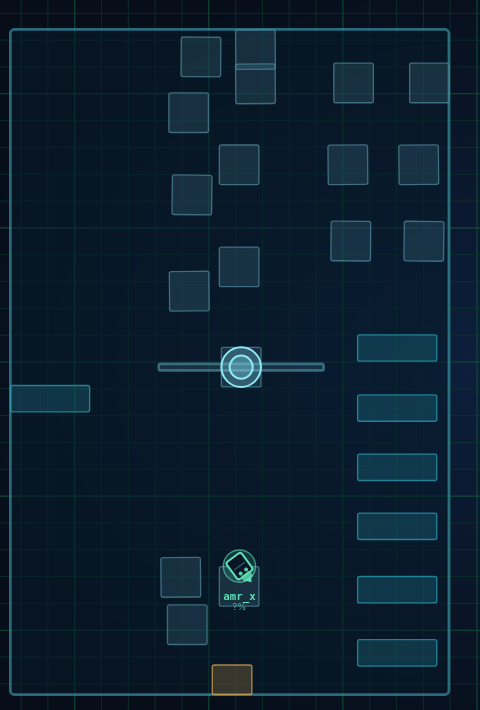
\includegraphics[width=\linewidth]{nav_web_before.png}
  \caption{Dashboard, avant.}
\end{subfigure}\hfill
\begin{subfigure}[b]{0.62\linewidth}\centering
  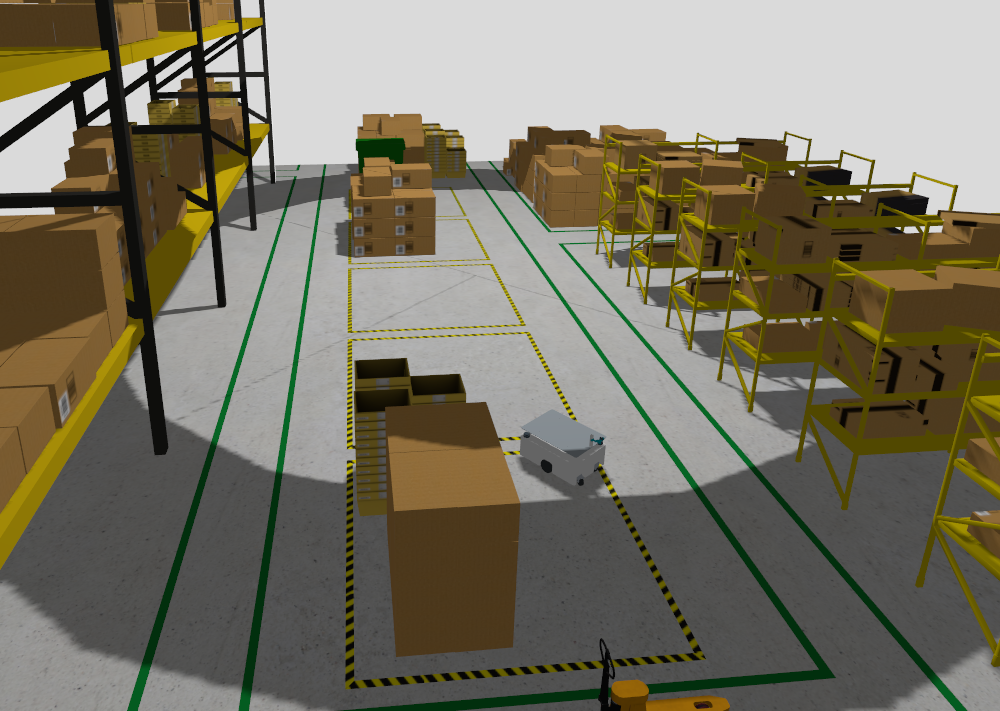
\includegraphics[width=\linewidth]{nav_gz_before.png}
  \caption{Gazebo, avant.}
\end{subfigure}\\[0.8em]
\begin{subfigure}[b]{0.34\linewidth}\centering
  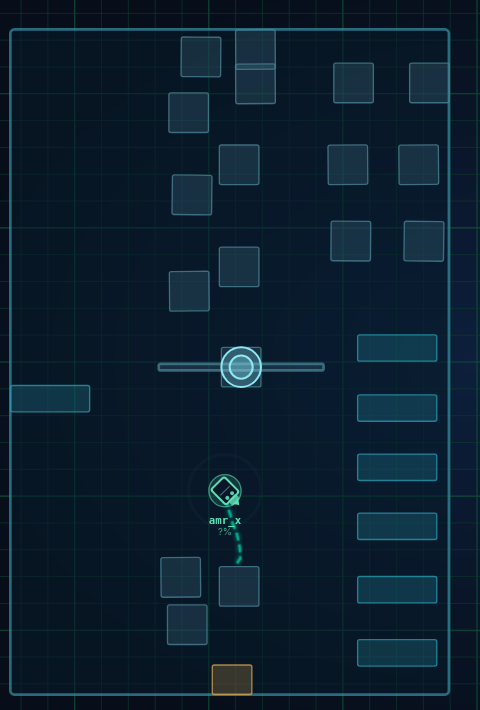
\includegraphics[width=\linewidth]{nav_web_after.png}
  \caption{Dashboard, après.}
\end{subfigure}\hfill
\begin{subfigure}[b]{0.62\linewidth}\centering
  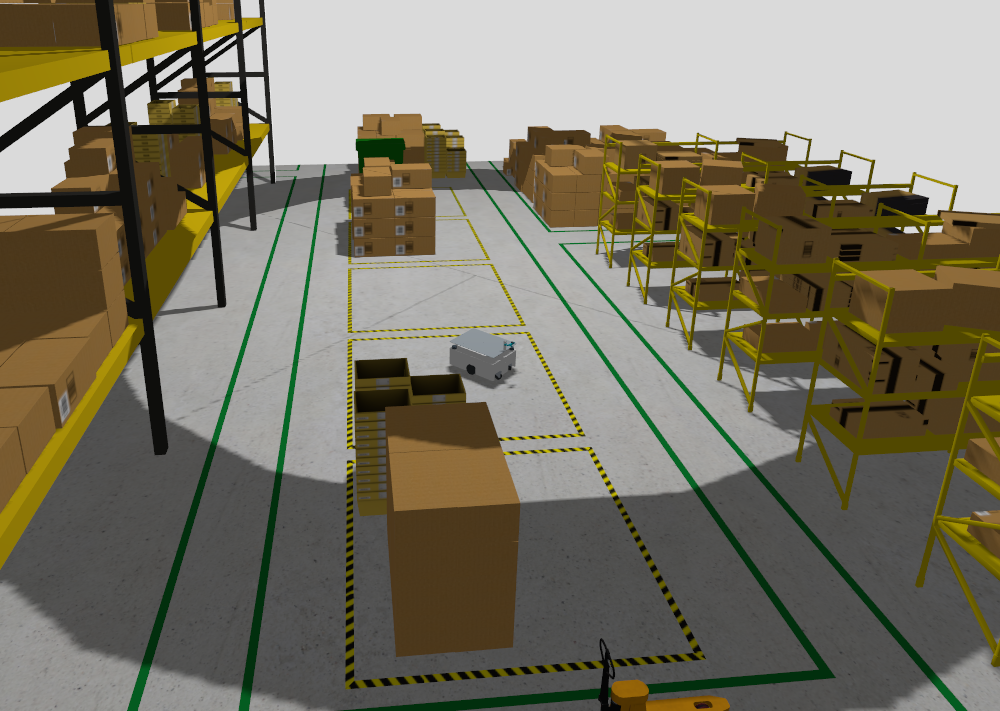
\includegraphics[width=\linewidth]{nav_gz_after.png}
  \caption{Gazebo, après.}
\end{subfigure}
\caption{Navigation réussie : déplacement du robot vu dans le dashboard et dans Gazebo.}
\label{fig:succes}
\end{figure}

\begin{figure}[htbp]
\centering

\includegraphics[width=0.7\linewidth]{nav_status_succeeded.png}
\caption{Résultat de la navigation affiché dans le panneau de flotte du dashboard.}
\label{fig:statut}
\end{figure}

\subsection{Analyse}
Les résultats montrent que la chaîne remplit les besoins fonctionnels : la destination
est acquittée immédiatement, la phase suit fidèlement l'exécution de Nav2 et la position
affichée correspond à celle du robot dans Gazebo à quelques centimètres près.

L'écart de cap final de 11° au scénario B reste inférieur à la tolérance angulaire
configurée dans Nav2 (\code{yaw\_goal\_tolerance} de 0,25~rad, soit 14,3°) ; de même,
l'erreur de position de 5,6~cm est inférieure à la tolérance de 0,25~m. Nav2 considère le
but atteint dès que ces tolérances sont respectées ; une précision plus fine relèverait du
réglage de Nav2 et non du dashboard.

La fréquence de l'état observée en temps réel (3,6 à 3,8~Hz) est légèrement inférieure aux
4~Hz nominaux. Le temporisateur de la passerelle étant cadencé sur le temps simulé, cette
fréquence suit la vitesse d'exécution de la simulation ; c'est aussi ce qui provoque l'arrêt
de la publication lorsque Gazebo est en pause, et donc le blocage des commandes dans le
dashboard après 2,5~s.

La latence d'acquittement mesurée (2~ms) a été obtenue par un client ROS local ; elle
n'inclut pas le passage par rosbridge et le navigateur.

\section{Points restant à valider}
Certains scénarios du protocole n'ont pas encore été exécutés dans la simulation :
\begin{itemize}
  \item \textbf{C} -- détour autour d'un obstacle : non mesuré spécifiquement ;
  \item \textbf{E} -- destination libre mais inaccessible : à réaliser pour vérifier que
    l'échec de Nav2 est bien affiché ;
  \item \textbf{H} -- coupure de rosbridge, puis reconnexion sans renvoi automatique ;
  \item \textbf{K} et \textbf{L} -- mode démonstration et changement d'adresse dans
    \emph{Settings}, vérifiés jusqu'ici par le test navigateur avec un faux serveur ROS
    uniquement ;
  \item cellule \emph{inconnue} : la costmap globale utilisée ne contenait aucune cellule
    inconnue ; ce cas n'est couvert que par les tests unitaires.
\end{itemize}
Ces essais doivent être conduits depuis l'interface web, en notant pour chacun la
configuration, le but, le résultat, la durée et les observations.

\section{Limites}
La solution est conçue pour la simulation. Elle ne gère qu'un robot et un monde à la
fois, n'arbitre pas les commandes venant d'autres sources (RViz, téléopération) et
n'ajoute pas d'authentification au niveau de rosbridge : elle n'est pas destinée à être
exposée sur un réseau ouvert. Fermer la page ou perdre la connexion n'arrête pas la
navigation en cours. Enfin, l'identifiant du monde et les décalages de repère sont
configurés par l'opérateur au lancement ; ils ne prouvent pas à eux seuls que le bon monde
et la bonne carte sont chargés, d'où l'intérêt de la vérification de position décrite
ci-dessus.

\section*{Conclusion}
Les essais en simulation ont permis de valider l'envoi de destinations, le suivi de
l'état, l'annulation, le refus des demandes invalides et la cohérence de la position
affichée. Ils ont aussi mis en évidence un décalage de 4,1~m entre la carte Nav2 et le
monde Gazebo, invisible sans comparaison avec la vérité terrain, qui a été analysé et
corrigé.

\chapter*{Conclusion générale et perspectives}
\addcontentsline{toc}{chapter}{Conclusion générale et perspectives}
\markboth{Conclusion générale et perspectives}{}

Ce stage avait pour objectif de permettre à un opérateur de commander le robot AMR-X
depuis le dashboard web du projet et d'y suivre fidèlement sa position et le résultat de
sa navigation. Au départ, le dashboard, la pile Nav2 et la simulation Gazebo
fonctionnaient séparément.

Pour les relier, une passerelle ROS~2 dédiée a été conçue et réalisée. Elle reçoit les
destinations par un service acquitté, vérifie chaque demande, dialogue avec Nav2 et publie
un état de navigation unique et versionné. Côté dashboard, la page \emph{Live map} permet
désormais de choisir une destination sur la carte ou par saisie, de l'envoyer, de suivre
la navigation et de l'annuler, tout en bloquant les commandes lorsque les données ne sont
plus fiables. Un script de lancement rend la chaîne complète reproductible en une seule
commande.

La validation en simulation a montré que la destination est acquittée immédiatement, que
l'état affiché suit l'exécution réelle de Nav2, que les demandes invalides ou concurrentes
sont refusées et que l'annulation arrête le robot. Elle a surtout mis en évidence un écart
de 4,1~m entre la position affichée et la position réelle du robot, dû à la différence
d'origine entre la carte SLAM et le monde Gazebo. Après mesure et configuration de ce
décalage, la position affichée dans le dashboard correspond à celle du robot dans Gazebo
à moins de 6~cm près. Ce résultat illustre l'importance de comparer l'interface à une
vérité terrain plutôt que de se fier à la seule cohérence interne du système.

Plusieurs perspectives se dégagent de ce travail :
\begin{itemize}
  \item terminer les scénarios restant à valider depuis l'interface (obstacle,
    destination inaccessible, coupure de rosbridge, mode démonstration, changement
    d'adresse) ;
  \item déterminer automatiquement le décalage entre la carte et le monde, par exemple en
    l'enregistrant avec la carte lors du SLAM, au lieu de le configurer à la main ;
  \item enregistrer les navigations lancées depuis la \emph{Live map} dans la base de
    données, afin de les relier à la gestion des missions ;
  \item étendre la passerelle à plusieurs robots et à l'arbitrage entre sources de
    commande ;
  \item sécuriser l'accès à rosbridge avant tout usage en dehors d'un poste de simulation,
    puis préparer le passage sur le robot physique.
\end{itemize}


\end{document}
